\chapter{Spectrum and Bandwidth Analysis}

\section{FFT and PSD}
The spectrum of the transmitted BPSK waveform is obtained using the Fast Fourier Transform (FFT). 
For a finite-duration BPSK signal, the spectrum is centered around the carrier frequency \(f_c\), 
and the signal exhibits the familiar bandpass shape of a modulated cosine waveform.

For the assigned parameters,
\[
f_c = 15~\text{kHz}, \qquad R_b = 1~\text{kbps}, \qquad f_s = 200~\text{kHz}
\]
the first spectral nulls of the BPSK spectrum occur at
\[
f_{L} = f_c - R_b = 15~\text{kHz} - 1~\text{kHz} = 14~\text{kHz}
\]
and
\[
f_{U} = f_c + R_b = 15~\text{kHz} + 1~\text{kHz} = 16~\text{kHz}
\]

Hence, the null-to-null bandwidth is
\[
BW = f_U - f_L = 2R_b = 2~\text{kHz}
\]

The power spectral density (PSD) of the waveform is obtained from the squared magnitude of the FFT, normalized by the signal length. The PSD shows how the signal power is distributed in frequency.

\section{Python Implementation}
The following code computes the FFT, plots the magnitude spectrum and PSD, and verifies Parseval's theorem.

\begin{lstlisting}[style=pythonstyle, caption={FFT and PSD Calculation for BPSK Signal}]
import numpy as np
import matplotlib.pyplot as plt

A = 1
fc = 15000
Rb = 1000
fs = 200000

Tb = 1 / Rb
t = np.arange(0, Tb, 1/fs)

s1 = A * np.cos(2 * np.pi * fc * t)
s0 = -A * np.cos(2 * np.pi * fc * t)

bits = np.array([1, 0, 1, 1, 0, 0, 1, 0, 1, 0])

waveform = np.array([])
for bit in bits:
    waveform = np.concatenate((waveform, s1 if bit == 1 else s0))

Nsig = len(waveform)
time_axis = np.arange(Nsig) / fs

X = np.fft.fftshift(np.fft.fft(waveform))
freq = np.fft.fftshift(np.fft.fftfreq(Nsig, d=1/fs))
PSD = (np.abs(X) ** 2) / Nsig

plt.figure(figsize=(12,4))
plt.plot(freq/1000, 20*np.log10(np.abs(X) + 1e-12))

plt.axvline(fc/1000, color='r', 
linestyle='--', 
label='Carrier frequency')

plt.axvline((fc-Rb)/1000, color='g', linestyle='--', label='Lower null')
plt.axvline((fc+Rb)/1000, color='m', linestyle='--', label='Upper null')
plt.xlabel('Frequency (kHz)')
plt.ylabel('Magnitude (dB)')
plt.title('FFT Magnitude Spectrum of BPSK Signal')
plt.grid(True)
plt.legend()
plt.tight_layout()
plt.show()

plt.figure(figsize=(12,4))
plt.plot(freq/1000, PSD, color='b')
plt.xlabel('Frequency (kHz)')
plt.ylabel('PSD')
plt.title('Power Spectral Density of BPSK Signal')
plt.grid(True)
plt.tight_layout()
plt.show()

E_time = np.sum(np.abs(waveform)**2) / fs
E_freq = np.sum(np.abs(X)**2) / (Nsig * fs)
error_percent = abs(E_time - E_freq) / E_time * 100

print("Time-domain energy =", E_time)
print("Frequency-domain energy =", E_freq)
print("Parseval error (%) =", error_percent)
print("Lower first null (kHz) =", (fc - Rb)/1000)
print("Upper first null (kHz) =", (fc + Rb)/1000)
print("Null-to-null bandwidth (kHz) =", 2*Rb/1000)
\end{lstlisting}
\newpage
\section{Bandwidth Calculation}
For BPSK, the null-to-null bandwidth is
\[
BW = 2R_b
\]
Substituting the assigned bit rate,
\[
BW = 2 \times 1~\text{kbps} = 2~\text{kHz}
\]

So the occupied main lobe lies approximately between \(14\) kHz and \(16\) kHz, centered at the carrier frequency of \(15\) kHz.

\section{Parseval Verification}
Parseval's theorem states that the signal energy in the time domain must equal the energy in the frequency domain:
\[
E_{\text{time}} = E_{\text{freq}}
\]

The percentage error is computed as
\[
\text{Error} = \frac{E_{\text{time}} - E_{\text{freq}}}{E_{\text{time}}}\times 100
\]

A very small error confirms that the discrete-time FFT implementation is correct and that the numerical signal representation preserves energy properly.

\section{Results and Discussion}
The FFT plot shows that the BPSK signal is concentrated around the carrier frequency \(15\) kHz, with the first nulls at \(14\) kHz and \(16\) kHz. This is consistent with the theoretical bandwidth relation \(BW=2R_b\).

The PSD plot gives a clearer view of signal power distribution and confirms that most of the useful energy lies inside the main spectral lobe. Since the waveform is digitally generated with finite duration, some spectral spreading is expected, but the dominant frequency structure still matches the theory.

\begin{figure}[htbp]
    \centering
    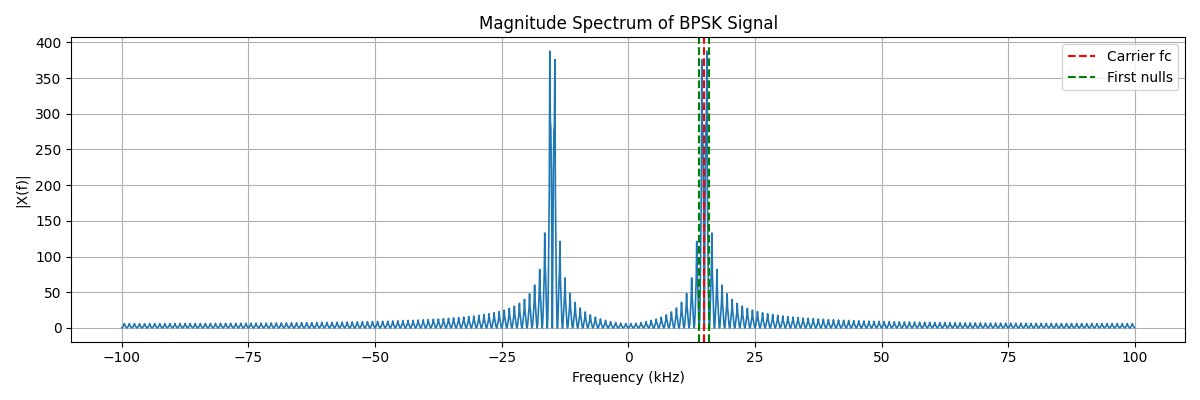
\includegraphics[width=0.8\textwidth]{plots/magnitude_spectrum_of_bpsk.png}
    \caption{FFT magnitude spectrum of the BPSK waveform}
\end{figure}

\begin{figure}[htbp]
    \centering
    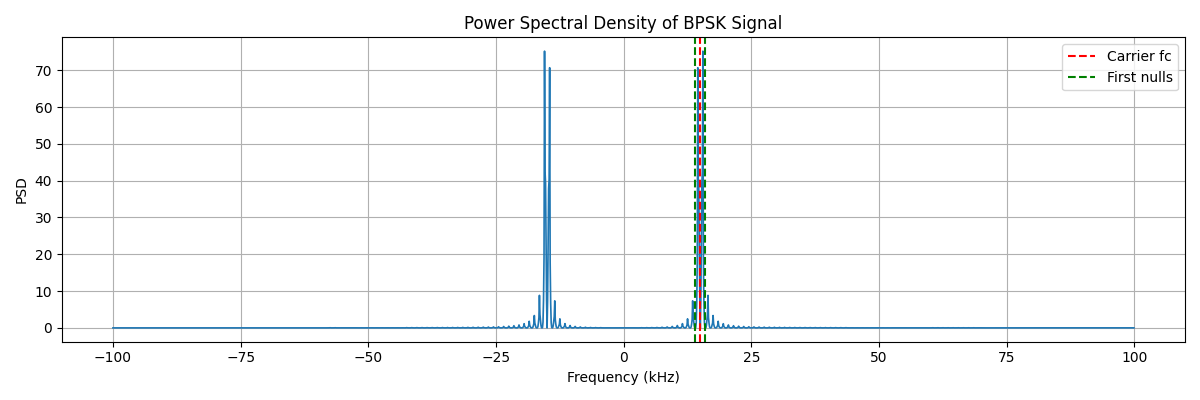
\includegraphics[width=0.8\textwidth]{plots/power_spectral_density_bpsk.png}
    \caption{Power spectral density of the BPSK waveform}
\end{figure}

The Parseval check should give a very small numerical error. \\This verifies that the sampled waveform and FFT scaling are implemented correctly, which is important before moving to channel modeling and BER simulation.